
% ================================================================
%  CAPITOLO 1 - LED
% ================================================================
\chapter{LED}

% ----------------------------------------------------------------
\section{Introduzione}

Il \textbf{LED} (\textit{Light Emitting Diode}, ovvero Diodo ad Emissione di Luce) è uno dei componenti elettronici più utilizzati al mondo. Lo troviamo ovunque nella vita  quotidiana: nei semafori stradali, nelle lampade a risparmio energetico, negli schermi  degli smartphone, nei display dei televisori, nelle luci dei cruscotti delle automobili  e persino nelle fibre ottiche che trasmettono dati su internet.

Il motivo del suo enorme successo è semplice: rispetto alle tradizionali lampadine a  incandescenza, il LED consuma molto meno energia, dura molto più a lungo (fino a  50.000 ore di funzionamento) e si accende istantaneamente senza surriscaldarsi.


% ----------------------------------------------------------------
\section{Struttura fisica e principio di funzionamento}
% ----------------------------------------------------------------

\subsection*{Cos'è un diodo}

Per capire un LED, dobbiamo prima capire cos'è un \textbf{diodo}. Un diodo è un  componente elettronico che permette alla corrente elettrica di scorrere \textbf{in una sola direzione}, bloccandola nell'altra. Si comporta come una valvola a senso unico per la corrente.

Questa proprietà è dovuta alla struttura interna del diodo, realizzata con materiali  \textbf{semiconduttori} (tipicamente il silicio o il germanio), ovvero materiali che si trovano a metà strada tra i conduttori (come il rame) e gli isolanti (come il vetro).

\subsection*{Perché un LED emette luce}

Un LED è un tipo particolare di diodo che, quando la corrente lo attraversa nel verso corretto, emette luce. Senza entrare nei dettagli della fisica quantistica, possiamo capirne il funzionamento con un'analogia intuitiva.

Immaginiamo gli elettroni come palline che si muovono all'interno del materiale semiconduttore. Quando una pallina \textit{cade} da un livello energetico alto a uno basso all'interno del materiale, rilascia energia. Nei normali resistori questa energia si trasforma in calore. In un LED, grazie alla scelta particolare dei materiali semiconduttori utilizzati (arseniuro di gallio, nitruro di gallio, ecc.), questa energia viene rilasciata sotto forma di \textbf{fotoni}, ovvero particelle di luce.

Il colore della luce emessa dipende direttamente dal materiale semiconduttore scelto: 
materiali diversi corrispondono a livelli energetici diversi, e quindi a colori diversi.

\begin{center}
\begin{tabular}{>{\bfseries}l l l}
    \toprule
    Colore & Materiale & Tensione tipica $V_f$ \\
    \midrule
    Rosso    & Arseniuro di gallio-alluminio (AlGaAs) & \SIrange{1.8}{2.1}{\volt} \\
    Arancione & Arseniuro di gallio-fosfuro (GaAsP)   & \SIrange{2.0}{2.2}{\volt} \\
    Giallo   & Fosfuro di gallio (GaP)                & \SIrange{2.1}{2.4}{\volt} \\
    Verde    & Nitruro di gallio-indio (InGaN)         & \SIrange{2.2}{3.5}{\volt} \\
    Blu      & Nitruro di gallio (GaN)                & \SIrange{3.0}{3.5}{\volt} \\
    Bianco   & LED blu + fosforo giallo               & \SIrange{3.0}{3.5}{\volt} \\
    \bottomrule
\end{tabular}
\end{center}

\begin{tcolorbox}[colback=blue!4, colframe=blue!60, title=\textbf{Curiosità: il LED bianco}]
    La luce bianca non esiste come singolo colore: è la sovrapposizione di tutti i 
    colori dello spettro. I LED bianchi vengono costruiti combinando un LED blu ad 
    alta efficienza con uno strato di materiale fosforescente giallo. La luce blu 
    eccita il fosforo che emette luce gialla; la combinazione di blu e giallo produce 
    la percezione del bianco da parte dell'occhio umano.
\end{tcolorbox}

\subsection*{Polarità del LED: anodo e catodo}

Come tutti i diodi, il LED è un componente \textbf{polarizzato}: ha un terminale positivo e uno negativo, e deve essere collegato nel verso giusto per funzionare.

\begin{itemize}
    \item \textbf{Anodo} (A): il terminale positivo. Si riconosce perché è la \textbf{gamba più lunga} del LED e all'interno del LED si nota che è presente una lamina chiamata \textbf{Lamina Minore}. Da questo terminale entra la corrente.
    \item \textbf{Catodo} (C): il terminale negativo. Si riconosce perché è la \textbf{gamba più corta} del LED e all'interno del LED si nota che è presente una lamina chiamata \textbf{Lamina Maggiore}. Da questo terminale esce la corrente.
\end{itemize}

\begin{figure}[h] % Ambiente float
    \centering
    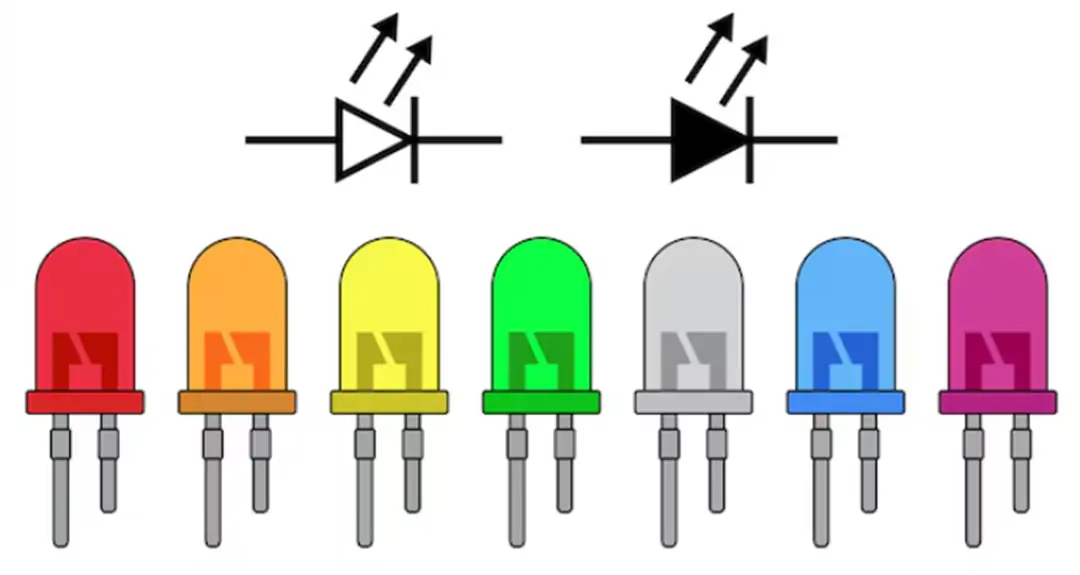
\includegraphics[width=0.7\textwidth]{img/Struttura_fisica_LED.png}
    \caption{Struttura fisica di un LED standard da 5mm.}
    \label{fig:struttura_fisica_LED}
\end{figure}

\begin{tcolorbox}[colback=red!4, colframe=red!60, title=\textbf{Attenzione - Polarità invertita}]
    Se colleghiamo il LED con la polarità invertita (provando a far entrare la corrente dal catodo), il LED \textbf{non si accende} e blocca il passaggio della corrente. In questa condizione il LED non si danneggia, ma semplicemente non funziona. Tuttavia, se la tensione inversa applicata supera il valore massimo specificato nel datasheet (tipicamente \SI{5}{\volt} per LED standard), il componente si danneggia irreversibilmente.
\end{tcolorbox}











% ----------------------------------------------------------------
\section{Parametri elettrici fondamentali}
% ----------------------------------------------------------------

Prima di collegare un LED a qualsiasi circuito, è indispensabile conoscere i suoi parametri elettrici. Questi valori si trovano nel \textbf{datasheet} del componente, ovvero la scheda tecnica fornita dal produttore.

\subsection*{Tensione di polarizzazione diretta \texorpdfstring{$V_f$}{Vf}}

La \textbf{tensione di polarizzazione diretta} (\textit{forward voltage}, $V_f$) è la caduta di tensione che si misura ai capi del LED quando è acceso e la corrente scorre nel verso corretto. Come abbiamo visto nella tabella precedente, questo valore dipende dal colore del LED e si aggira tipicamente tra \SI{1.8}{\volt} e \SI{3.5}{\volt}.

È fondamentale ricordare che $V_f$ è una \textbf{proprietà fisica del componente}: non possiamo cambiarla. Qualunque sia la tensione di alimentazione del nostro circuito, la differenza di potenziale ai capi del LED \textit{sarà sempre e solo} la sua $V_f$.

\subsection*{Corrente diretta nominale \texorpdfstring{$I_f$}{If}}

La \textbf{corrente diretta nominale} (\textit{forward current}, $I_f$) è il valore di corrente per cui il LED è stato progettato per funzionare in modo ottimale e sicuro. Per i LED standard da 5 mm (quelli che useremo con Arduino), questo valore è tipicamente \SI{20}{\milli\ampere}.

\begin{tcolorbox}[colback=red!4, colframe=red!60, title=\textbf{Perché la corrente è così critica?}]
    A differenza di una resistenza, il LED \textbf{non limita autonomamente la corrente 
    che lo attraversa}. Se lo colleghiamo direttamente a una sorgente di tensione, la 
    corrente tenderebbe ad aumentare senza controllo fino a distruggere il componente 
    in pochi millisecondi. Per questo motivo è \textbf{sempre obbligatorio} inserire 
    una resistenza di limitazione in serie al LED.
\end{tcolorbox}

\subsection*{Corrente massima assoluta}

La \textbf{corrente massima assoluta} è il valore oltre il quale il LED si danneggia 
in modo permanente e istantaneo. Per i LED standard è circa \SI{30}{\milli\ampere}. 
Non si deve mai avvicinarsi a questo valore: in pratica, per un uso sicuro con Arduino, 
è consigliabile lavorare con correnti tra \SI{5}{\milli\ampere} e \SI{15}{\milli\ampere}.

\begin{tcolorbox}[colback=blue!4, colframe=blue!60, title=\textbf{Nota pratica}]
    I pin digitali di Arduino Uno possono erogare al massimo \SI{40}{\milli\ampere} per poco tempo, ma la scheda nel suo complesso non dovrebbe superare \SI{200}{\milli\ampere} totali. Per sicurezza, è buona norma progettare i circuiti per non superare i \SI{10}{\milli\ampere} per LED.
\end{tcolorbox}
















% ----------------------------------------------------------------
\section{La resistenza di limitazione}
% ----------------------------------------------------------------

\subsection*{Perché è necessaria}

Abbiamo visto che il LED non può essere collegato direttamente alla tensione di 
alimentazione perché la corrente diventerebbe eccessiva. La soluzione è inserire 
in \textbf{serie} al LED una \textbf{resistenza di limitazione} $R$, il cui compito 
è quello di \textit{assorbire} la differenza di tensione tra l'alimentazione e la 
$V_f$ del LED, limitando di conseguenza la corrente.

\subsection*{Calcolo con la legge di Kirchhoff e la legge di Ohm}

Consideriamo il circuito in serie composto da: sorgente di tensione $V_{cc}$, 
resistenza $R$ e LED con tensione $V_f$.

Applicando la \textbf{legge di Kirchhoff alle tensioni} (la somma delle tensioni in 
un anello chiuso è zero), otteniamo:

\begin{equation}
    V_{cc} = V_R + V_f
\end{equation}

Un altro modo per vedere questa equazione è pensare che la tensione totale fornita da $V_{cc}$ si divide tra la resistenza e il LED. La tensione che cade sulla resistenza, $V_R$, è quindi:

\begin{equation}
    V_R = V_{cc} - V_f
\end{equation}

In un circuito in serie la corrente è uguale in ogni punto, quindi la corrente che attraversa la resistenza è la stessa che attraversa il LED: $I_R = I_f$.\\
Applicando la \textbf{legge di Ohm} alla resistenza ($V = R \cdot I$):

\begin{equation}
    R = \frac{V_R}{I_f} = \frac{V_{cc} - V_f}{I_f}
\end{equation}

\subsection*{Esempio di calcolo}

Vogliamo collegare un \textbf{LED rosso} al pin 13 di Arduino, che fornisce 
\SI{5}{\volt}. Il LED rosso ha $V_f = \SI{2.0}{\volt}$ e vogliamo farlo 
lavorare a $I_f = \SI{10}{\milli\ampere}$ per sicurezza.

\begin{equation}
    R = \frac{V_{cc} - V_f}{I_f} = \frac{\SI{5}{\volt} - \SI{2.0}{\volt}}{\SI{10}{\milli\ampere}} = \frac{\SI{3}{\volt}}{\SI{0.010}{\ampere}} = \SI{300}{\ohm}
\end{equation}

Il valore esatto di \SI{300}{\ohm} potrebbe non essere disponibile nella serie 
standard di resistenze commerciali. In questo caso scegliamo il valore 
\textbf{immediatamente superiore} disponibile, cioè \textbf{\SI{330}{\ohm}}: 
una resistenza leggermente più alta riduce leggermente la corrente (e quindi la 
luminosità), ma protegge meglio il componente. Non si sceglie mai un valore 
inferiore, perché aumenterebbe la corrente oltre il valore di progetto.

\begin{tcolorbox}[colback=olive!4, colframe=olive!60, title=\textbf{Verifica del calcolo}]
    Con $R = \SI{330}{\ohm}$, la corrente effettiva sarà:
    \[
        I_f = \frac{V_{cc} - V_f}{R} = \frac{\SI{5}{\volt} - \SI{2.0}{\volt}}{\SI{330}{\ohm}} \approx \SI{9.1}{\milli\ampere}
    \]
    Valore ben al di sotto dei \SI{20}{\milli\ampere} nominali: il LED è al sicuro.
\end{tcolorbox}

\section{Schema di collegamento}
% ----------------------------------------------------------------

\subsection*{Componenti necessari}

\begin{center}
\begin{tabular}{>{\bfseries}l l}
    \toprule
    Q.tà & Materiale \\
    \midrule
    1 & Generatore di tensione (es. Arduino Uno/Mega)  \\
    2 & LED (colore a scelta)  \\
    2 & Resistori \\
    1 & Breadboard   \\
    vari  & Cavi e Jumpers  \\
    \bottomrule
\end{tabular}
\end{center}

\subsection*{Schema elettrico}

\begin{figure}[h]
    \centering
    \begin{minipage}{0.5\textwidth}  % Larghezza della minipagina per l'immagine
        \centering
        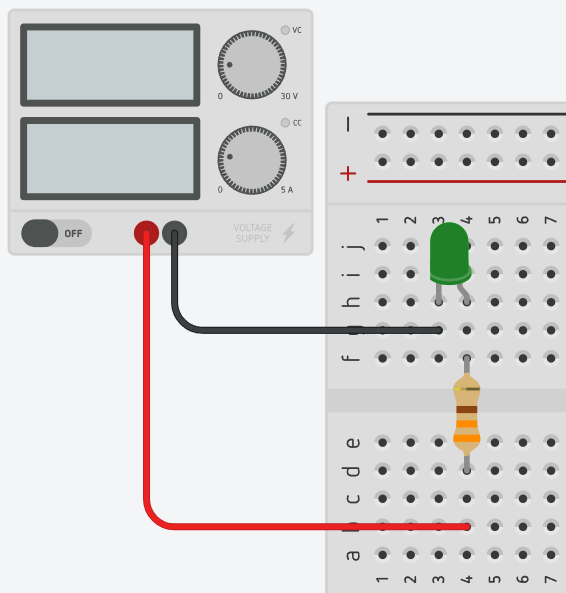
\includegraphics[width=0.8\textwidth]{img/Circuito_LED_Generatore.png}
        \caption{\centering Circuito elettrico realizzato su Tinkercad.}
        \label{fig:Circuito_LED_Generatore}
    \end{minipage}%
    \hfill
    \begin{minipage}{0.45\textwidth}  % Larghezza della minipagina per il circuito
        \centering
        \begin{circuitikz}[scale=1.6, american]
            %\draw[help lines,red,thin,dotted] (0,0) grid (5,5);
            \draw (0,0)
                to[short] (0,0)
                to[R, l=R] (0,-2)
                to[led, l=LED] (0,-4)
                to[short] (-2,-4)
                to[V, l=$E$, invert] (-2,0)
                to[short] (0,0);
            \node[below] at (-0.15,-2.5) {\texttt{A}};
            \node[below] at (-0.15,-3.2) {\texttt{C}};
        \end{circuitikz}
        \caption{Schema elettrico.}
        \label{fig:Schema_LED}
    \end{minipage}
\end{figure}

Nelle figure (\ref{fig:Circuito_LED_Generatore}) e (\ref{fig:Schema_LED}) vediamo lo schema elettrico per accendere un LED con un generatore di tensione. Il terminale positivo del generatore è collegato all'anodo del LED attraverso una resistenza di limitazione, mentre il catodo del LED è collegato al terminale negativo del generatore.
Dato che nell'esempio abbiamo scelto un LED verde, possiamo supporre che la tensione di polarizzazione diretta sia $V_f = \SI{2.6}{\volt}$ e che la corrente nominale sia $I_f = \SI{20}{\milli\ampere}$. Se il generatore fornisce $V_{cc} = \SI{5}{\volt}$, la resistenza di limitazione da inserire in serie al LED sarà:

\begin{equation}
    R = \frac{V_{cc} - V_f}{I_f} = \frac{\SI{5}{\volt} - \SI{2.6}{\volt}}{\SI{20}{\milli\ampere}} = \frac{\SI{2.4}{\volt}}{\SI{0.020}{\ampere}} = \SI{120}{\ohm}
\end{equation}

Una resistenza di \SI{120}{\ohm} potrebbe non essere disponibile, quindi scegliamo il valore commerciale più vicino e superiore, cioè \textbf{\SI{150}{\ohm}}, che garantisce una corrente di $\SI{16}{\milli\ampere}$, leggermente inferiore a quella nominale, ma comunque sufficiente per accendere il LED in modo visibile.\\



Se il circuito viene fatto utilizzando come generatore di tensione una scheda Arduino, è sempre meglio aumentare il valore di resistenza  $\SIrange{220}{330}{\ohm}$, in maniera da non stressare troppo i pin digitali di Arduino. Per verificare se il circuito è fatto correttamente, basta collegare il jumper che abbiamo precedentemente collegato alla boccola positiva dell'alimentatore al pin \texttt{+5\,V} e collegare il jumper che abbiamo precedentemente collegato alla boccola negativa dell'alimentatore al pin \texttt{GND} di Arduino. Se tutto è stato fatto correttamente, il LED si accenderà. Se il led non si accende allora bisogna controllare se il circuito è stato montato correttamente prestando attenzione ai vari collegamenti sulla breadboard e alla polarità del LED. Se continua a non accendersi se la resistenza che abbiamo scelto non sia troppo alta, oppure che il LED non sia danneggiato.

\begin{figure}[h]
    \centering
    \begin{minipage}{0.55\textwidth}  % Larghezza della minipagina per l'immagine
        \centering
        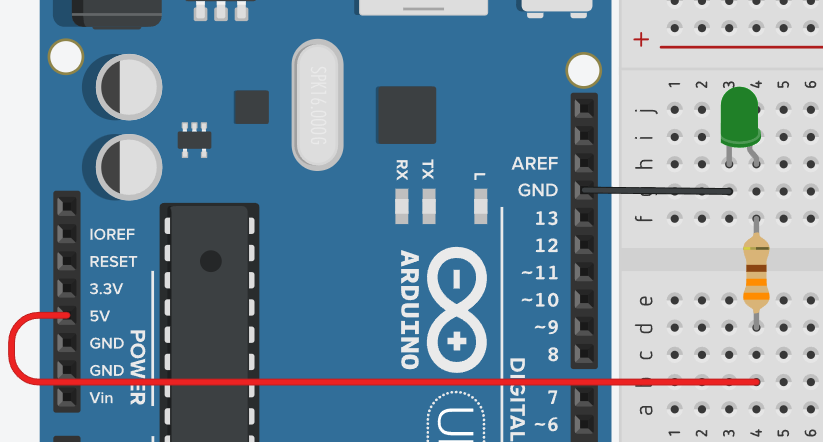
\includegraphics[width=\textwidth]{img/Circuito_Led_5V.png}
        \caption{\centering Circuito per verificare\protect\\ il funzionamento del circuito.}
        \label{fig:Circuito_LED_5V}
    \end{minipage}%
    \hfill
    \begin{minipage}{0.45\textwidth}  % Larghezza della minipagina per l'immagine
        \centering
        \includegraphics[width=0.6\textwidth]{img/Circuito_Led_Arduino.png}
        \caption{\centering Circuito per accendere \protect\\il LED con Arduino.}
        \label{fig:Circuito_LED_Arduino}
    \end{minipage}%
\end{figure}






\section{LED RGB}
% ----------------------------------------------------------------

Il \textbf{LED RGB} è un componente che racchiude all'interno dello stesso componente tre LED: uno Rosso (\textit{Red}), uno Verde (\textit{Green}) e uno Blu (\textit{Blue}). Controllando separatamente l'intensità di ciascuno di essi è possibile generare un'ampia gamma di colori, sfruttando il principio della sintesi additiva dei colori.

\subsection*{Struttura interna e tipologie}

Un LED RGB ha quattro terminali: tre anodi (uno per ciascun colore) e un catodo comune, oppure tre catodi e un anodo comune. Le due configurazioni possibili sono:

\begin{itemize}
    \item \textbf{Anodo comune} (Common Anode): tutti e tre gli anodi sono collegati insieme al terminale positivo. Per accendere un colore, si porta a massa (GND) il catodo corrispondente.
    \item \textbf{Catodo comune} (Common Cathode): tutti e tre i catodi sono collegati insieme al terminale negativo. Per accendere un colore, si applica una tensione positiva all'anodo corrispondente.

\end{itemize}
\begin{tcolorbox}[colback=blue!4, colframe=blue!60, title=\textbf{Quale usare con Arduino?}]
    La maggior parte dei kit didattici utilizza LED RGB a \textbf{catodo comune}. In questo caso il pin comune va collegato a GND, e i tre pin dei colori vanno collegati ad Arduino attraverso tre resistenze di limitazione (una per canale). Per un LED RGB ad anodo comune, il pin comune va collegato a \SI{5}{\volt} e i pin dei colori vanno portati a GND per accendere il LED (logica invertita).
\end{tcolorbox}

\subsection*{Generazione dei colori}

I tre LED interni possono essere accesi singolarmente o in combinazione. La tabella seguente mostra i colori ottenuti accendendo a piena intensità diverse combinazioni (per catodo comune):

\begin{center}
\begin{tabular}{>{\bfseries}l c c c c}
    \toprule
    Colore risultante & Rosso (R) & Verde (G) & Blu (B) \\
    \midrule
    Rosso    & HIGH  & \textcolor{lightgray}{LOW} & \textcolor{lightgray}{LOW} \\
    Verde    & \textcolor{lightgray}{LOW} & HIGH  & \textcolor{lightgray}{LOW} \\
    Blu      & \textcolor{lightgray}{LOW} & \textcolor{lightgray}{LOW} & HIGH  
    \vspace{0.4cm}\\
    
    Ciano    & \textcolor{lightgray}{LOW} & HIGH  & HIGH  \\
    Magenta  & HIGH  & \textcolor{lightgray}{LOW} & HIGH \\
    Giallo   & HIGH  & HIGH  & \textcolor{lightgray}{LOW} 
        \vspace{0.4cm}\\
    Bianco   & HIGH  & HIGH  & HIGH  \\
    Spento   & \textcolor{lightgray}{LOW} & \textcolor{lightgray}{LOW} & \textcolor{lightgray}{LOW} \\
    \bottomrule
\end{tabular}
\end{center}

Variando l'intensità di ciascun canale tramite PWM si ottengono infinite sfumature. Ad esempio, un rosso intenso si ottiene con R=255, G=0, B=0; un arancione si può ottenere con R=255, G=80, B=0. Potendo usare 256 livelli di intensità per ciascun colore del LED RGB, si possono generare $256^3 = 16.777.216$ combinazioni diverse.

\subsection*{Schema di collegamento}

Colleghiamo un LED RGB a catodo comune ai pin digitali di Arduino. Utilizziamo tre resistenze di limitazione, una per ogni colore. Il calcolo della resistenza è identico a quello visto per il LED singolo, usando la $V_f$ di ogni colore (tipicamente: rosso $\SI{2.0}{\volt}$, verde $\SI{2.2}{\volt}$, blu $\SI{3.2}{\volt}$). Per semplicità, con alimentazione a \SI{5}{\volt} e una corrente di circa \SI{10}{\milli\ampere}, si possono usare resistenze da \SI{330}{\ohm} per tutti e tre i canali.

\begin{figure}[h]
    \centering
    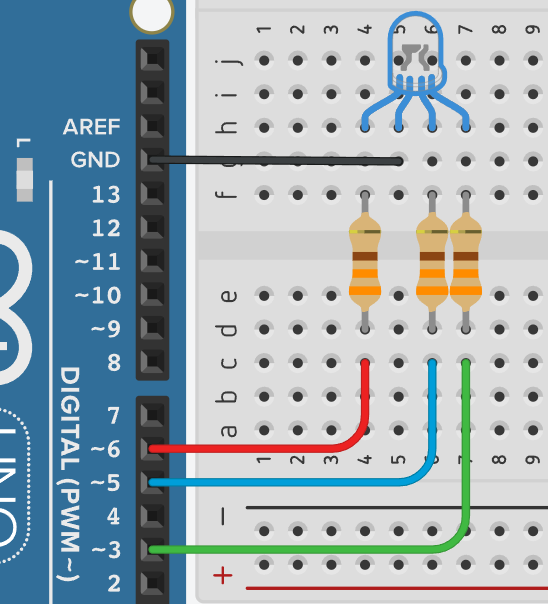
\includegraphics[width=0.35\textwidth]{img/LED_RGB.png}
    \caption{Schema di collegamento di un LED RGB a catodo comune con Arduino.}
    \label{fig:LED_RGB_Arduino}
\end{figure}

Ricordiamo che per poter controllare la luminosità di ciascun colore è necessario utilizzare i pin digitali con funzionalità PWM e la funzione \texttt{analogWrite()} per variare il duty cycle del segnale.


























% ----------------------------------------------------------------
\section{Programmazione con Arduino}
% ----------------------------------------------------------------

\subsection*{Configurare un pin come uscita: \texttt{pinMode()}}

Prima di poter controllare un LED (o qualsiasi altro componente), dobbiamo dire ad Arduino se quel pin digitale deve comportarsi da \textbf{uscita} (Arduino manda tensione al circuito) o da \textbf{ingresso} (Arduino legge la tensione dal circuito). 
Questo si fa con la funzione che dichiara la modalità di utilizzo del pin, cioè la funzione \texttt{pinMode()}:

\begin{center}
    \hrule
    \vspace{0.2cm}
    \texttt{pinMode(numeroPIN, modalità);}
    \vspace{0.2cm}
    \hrule
\end{center}

\begin{itemize}
    \item \texttt{numeroPIN}: il numero del pin da configurare (es. \texttt{6}, come mostrato in figura \ref{fig:Circuito_LED_Arduino})
    \item \texttt{modalità}: \texttt{OUTPUT} per uscita, \texttt{INPUT} per ingresso. Per accendere un LED, bisogna inviare un segnale dall'Arduino all' "esterno", quindi configureremo il pin come pin di \texttt{OUTPUT}.
\end{itemize}

Quindi per impostare il pin 6 come pin usato per accendere il led in figura \ref{fig:Circuito_LED_Arduino} bisogna scrivere:
\begin{center}
    \hrule
    \vspace{0.2cm}
    \texttt{pinMode(6, OUTPUT);}
    \vspace{0.2cm}
    \hrule
\end{center}

\subsection*{Accendere e spegnere il LED: \texttt{digitalWrite()}}

Per portare un pin digitale a \SI{5}{\volt} (LED acceso) o a \SI{0}{\volt} 
(LED spento) si usa \texttt{digitalWrite()}:

\begin{center}
    \hrule
    \vspace{0.2cm}
\texttt{digitalWrite(numeroPIN, valore);}
    \vspace{0.2cm}
    \hrule
\end{center}

\begin{itemize}
    \item \texttt{HIGH}: porta il pin a \SI{5}{\volt} → LED \textbf{acceso}
    \item \texttt{LOW}: porta il pin a \SI{0}{\volt} → LED \textbf{spento}
\end{itemize}

Quindi per accendere il LED collegato al pin 6 bisogna scrivere:
\begin{center}
    \hrule
    \vspace{0.2cm}
    \texttt{digitalWrite(6, HIGH);}
    \vspace{0.2cm}
    \hrule
\end{center}

Mentre per spegnere il led bisognerà scrivere:

\begin{center}
    \hrule
    \vspace{0.2cm}
    \texttt{digitalWrite(6, LOW);}
    \vspace{0.2cm}
    \hrule
\end{center}



\subsection{Lampeggio del LED e funzione \texttt{delay/(ms);}}

Proviamo subito a far lampeggiare un LED, accendendolo e spegnendolo all'interno della funzione \texttt{void loop()}. Abbiamo anche bisogno di dichiarare che il pin dove verrà collegato il LED è un pin di \texttt{OUTPUT}, quindi scriveremo \texttt{pinMode()} all'interno della funzione \texttt{void setup()}.
Quindi il codice completo per far lampeggiare un LED collegato al pin 6 dovrebbe essere il seguente:

\begin{tcblisting}{
    listing only,
    listing engine=listings,
    colback=red!5,
    colframe=red!50,
    title=\textbf{Esempio 1 - Blink NON funzionante},
    breakable,
    listing options={
        language=C++,
        basicstyle=\ttfamily\small,
        keywordstyle=\color{blue!80!black}\bfseries,
        commentstyle=\color{green!50!black}\itshape,
        stringstyle=\color{orange!80!black},
        numbers=left,
        numberstyle=\tiny\color{gray},
        breaklines=true,
        showstringspaces=false,
        morekeywords={pinMode, digitalWrite, delay, OUTPUT, HIGH, LOW, void, const, int}
    }
}
void setup() {
    pinMode(6, OUTPUT);
}

void loop() {
    digitalWrite(6, HIGH);  // Accende LED (porta il pin a 5V)
    digitalWrite(6, LOW);   // Spegne LED (porta il pin a 0V)
}
\end{tcblisting}

Se proviamo a caricare questo \textit{sketch} su Arduino, vedremo che il funzionamento atteso non rispecchia quello che stiamo notando sul nostro LED: il LED si accende e si spegne così rapidamente che sembra essere sempre acceso. 
Ricordiamo che la funzione \texttt{void loop()} viene eseguita in modo continuo e ciclico, quindi il LED viene acceso e spento migliaia di volte al secondo. Questa velocità di esecuzione è troppo elevata per essere percepita dall'occhio umano, che appunto vede il LED sempre acceso.

Per risolvere questo problema, dobbiamo inserire una pausa tra l'accensione e lo spegnimento del LED. La funzione \texttt{delay()} ci permette di bloccare l'esecuzione del programma per un certo numero di \textbf{millisecondi}. Se vogliamo che il LED rimanga acceso per 1 secondo e poi spento per 1 secondo, dobbiamo inserire un \texttt{delay(1000);} dopo ogni comando di accensione o spegnimento.\\

Inoltre, aggiungiamo in questo codice una riga per creare una variabile che contiene il numero del pin a cui è collegato il LED, in modo da rendere il codice più leggibile e facilmente modificabile in futuro.

\begin{tcblisting}{
    listing only,
    listing engine=listings,
    colback=teal!5,
    colframe=teal!50,
    title=\textbf{Esempio 2 - Blink},
    breakable,
    listing options={
        language=C++,
        basicstyle=\ttfamily\small,
        keywordstyle=\color{blue!80!black}\bfseries,
        commentstyle=\color{green!50!black}\itshape,
        stringstyle=\color{orange!80!black},
        numbers=left,
        numberstyle=\tiny\color{gray},
        breaklines=true,
        showstringspaces=false,
        morekeywords={pinMode, digitalWrite, delay, OUTPUT, HIGH, LOW, void, const, int}
    }
}
const int ledPin = 6;  // Pin a cui è collegato il LED

void setup() {
    pinMode(ledPin, OUTPUT);
}

void loop() {
    digitalWrite(ledPin, HIGH);
    delay(1000);          // Aspetta 1000 millisecondi (1 secondo)
    digitalWrite(ledPin, LOW);
    delay(1000);          // Aspetta 1000 millisecondi (1 secondo)
}
\end{tcblisting}


\textbf{Analisi del codice riga per riga:}
\begin{itemize}
    \item \textbf{Riga 1} - \texttt{const int ledPin = 6;}: dichiara una variabile costante di tipo intero chiamata \texttt{ledPin} e le assegna il valore 6, che rappresenta il numero del pin digitale a cui è collegato il LED.
    \begin{itemize}
        \item \texttt{int} indica che la variabile è di tipo intero
        \item \texttt{const} indica che il valore di questa variabile non può essere modificato durante l'esecuzione del programma, se per errore si tenta di assegnare un nuovo valore a \texttt{ledPin}, il compilatore genererà un errore, proteggendo così la costante da modifiche accidentali.
        \item L'uso di una variabile con nome significativo come \texttt{ledPin} rende il codice più leggibile e facile da capire, rispetto a usare direttamente il numero 6 in tutto il programma. Si può facilmente modificare il numero del pin in un solo punto (la dichiarazione della variabile) se si decide di collegare il LED a un pin diverso in futuro, senza dover cercare e sostituire ogni occorrenza del numero 6 nel codice.
    \end{itemize}
    , mentre 
    \item \textbf{Riga 4} - \texttt{pinMode(ledPin, OUTPUT);}: eseguita una sola volta all'avvio, configura il pin ledPin come uscita digitale.
    \item \textbf{Riga 8} - \texttt{digitalWrite(ledPin, HIGH);}: porta il pin 13 a \SI{5}{\volt}. La corrente scorre attraverso la resistenza e il LED, che si accende.
    \item \textbf{Riga 9 e Riga 11} - \texttt{delay(1000);}: il programma si blocca per 1000 ms. Durante questo tempo il LED rimane nello stato in cui si trova.
    \item \textbf{Riga 10} - \texttt{digitalWrite(ledPin, LOW);}: porta il pin ledPin a \SI{0}{\volt}. Nessuna differenza di tensione, nessuna corrente, LED spento.
\end{itemize}

\subsection{Variare la luminosità: PWM e \texttt{analogWrite()}}

I pin digitali di Arduino possono essere solo in due stati: \SI{5}{\volt} \texttt{(HIGH)} oppure \SI{0}{\volt} \texttt{(LOW)} . Non è possibile impostare direttamente una tensione intermedia di, ad esempio, \SI{2.5}{\volt}. Come facciamo allora a variare la luminosità del LED?\\

La soluzione si chiama \textbf{PWM} (\textit{Pulse Width Modulation}, Modulazione di Larghezza di Impulso). L'idea è la seguente: invece di tenere il pin fisso a un valore di tensione intermedio, il pin viene commutato rapidamente tra HIGH e LOW a una frequenza molto alta. L'occhio umano, non riuscendo a percepire variazioni così rapide, vede una luminosità \textit{media} che da l'impressione di essere proporzionale al tempo in cui il pin è rimasto HIGH.\\

Questo rapporto tra il tempo $t_{\texttt{H}}$ in cui il segnale è \texttt{HIGH} e il periodo totale si chiama 
\textbf{duty cycle}:

\begin{equation}
    \text{Duty Cycle} = \frac{t_{\texttt{H}}}{T} \times 100\%
\end{equation}

Un duty cycle del 50\% significa che il pin è \texttt{(HIGH)} per metà del tempo: il LED appare a metà della sua luminosità massima. Un duty cycle del 100\% equivale a \texttt{digitalWrite(pin, HIGH)}: LED alla massima luminosità.

\begin{center}
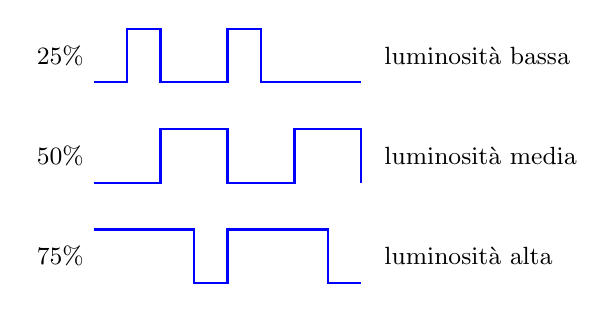
\begin{tikzpicture}[scale=0.85]
    % Duty cycle 25%
    \node[left] at (0,3.4) {\small 25\%};
    \draw[thick, blue] (0,3) -- (0.5,3) -- (0.5,3.8) -- (1,3.8) -- (1,3) -- (2,3) -- (2,3.8) -- (2.5,3.8) -- (2.5,3) -- (4,3);
    % Duty cycle 50%
    \node[left] at (0,1.9) {\small 50\%};
    \draw[thick, blue] (0,1.5) -- (1,1.5) -- (1,2.3) -- (2,2.3) -- (2,1.5) -- (3,1.5) -- (3,2.3) -- (4,2.3) -- (4,1.5);
    % Duty cycle 75%
    \node[left] at (0,0.4) {\small 75\%};
    \draw[thick, blue] (0,0.8) -- (1.5,0.8) -- (1.5,0) -- (2,0) -- (2,0.8) -- (3.5,0.8) -- (3.5,0) -- (4,0);
    % titolo
    \node[right] at (4.2,3.4) {\small luminosità bassa};
    \node[right] at (4.2,1.9) {\small luminosità media};
    \node[right] at (4.2,0.4) {\small luminosità alta};
\end{tikzpicture}
\end{center}

La funzione \texttt{analogWrite(pin, valore);} imposta il duty cycle del pin PWM specificato. Il parametro \texttt{valore} va da \textbf{0} (duty cycle 0\%, LED completamente spento) a \textbf{255} (duty cycle 100\%, LED alla massima  luminosità). Se quindi vogliamo accendere il LED al 32\% dobbiamo ricorrere as una semplice proporzione:
\begin{equation}
    \texttt{valore} : 255 = 32 : 100 \qquad \implies \qquad \texttt{valore} = \frac{32}{100} \times 255 \approx 82
\end{equation}
Il numero massimo di 255 è dovuto al fatto che il duty cycle viene rappresentato internamente con un numero a 8 bit (1 byte), che può assumere 256 valori (da 0 a 255).
\begin{tcolorbox}[colback=orange!4, colframe=orange!70, title=\textbf{Quali pin supportano il PWM?}]
    Su Arduino Uno, \textbf{non tutti i pin} supportano il PWM. I pin abilitati al PWM sono contrassegnati dal simbolo \textbf{$\sim$} sulla scheda e sono: \textbf{3, 5, 6, 9, 10, 11}. Se si tenta di usare \texttt{analogWrite()} su un pin non PWM, il comportamento è imprevedibile.
\end{tcolorbox}
\begin{tcolorbox}[colback=red!4, colframe=red!60, title=\textbf{analogWrite non vuol dire pin analogico!}]
    \texttt{analogWrite();} è una funzione che si applica solo ai pin digitali abilitati al PWM, non ai pin analogici. I pin analogici di Arduino (quelli identificati con una A e un numero) sono progettati solamente per leggere segnali analogici (con \texttt{analogRead()}) e non possono essere usati per generare un segnale PWM.
\end{tcolorbox}



Quindi possiamo ora scrivere un programma che accende un LED al 20\% di luminosità per 1 secondo, poi lo spegne, poi lo riaccende ma al 80\% di luminosità per 1 secondo, poi lo rispegne e così via:

\begin{tcblisting}{
    listing only,
    listing engine=listings,
    colback=teal!5,
    colframe=teal!50,
    title=\textbf{Esempio 3 - Variazione luminosità},
    breakable,
    listing options={
        language=C++,
        basicstyle=\ttfamily\small,
        keywordstyle=\color{blue!80!black}\bfseries,
        commentstyle=\color{green!50!black}\itshape,
        stringstyle=\color{orange!80!black},
        numbers=left,
        numberstyle=\tiny\color{gray},
        breaklines=true,
        showstringspaces=false,
        morekeywords={pinMode, analogWrite, digitalWrite, delay, OUTPUT, HIGH, LOW, void, const, int}
    }
}
const int pinLed = 6;

void setup() {
  pinMode(pinLed, OUTPUT);
}

void loop() {
    analogWrite(pinLed, 51);  // Accende il LED con duty cycle 20 %
    delay(1000);               
    analogWrite(pinLed, 0);   // Spegne il LED con duty cycle 0 %
    delay(1000);               
    analogWrite(pinLed, 204); // Accende il LED con duty cycle 80 %
    delay(1000);              
    analogWrite(pinLed, 0);   // Spegne il LED con duty cycle 0 %
    delay(1000);              
}
\end{tcblisting}


\subsection{LED RGB}

Grazie al PWM possiamo controllare non solo la luminosità di un singolo LED, ma anche il colore di un LED RGB, miscelando in proporzioni variabili l'intensità dei tre canali Rosso, Verde e Blu.

\subsubsection*{Accendere un colore primario}

Per ottenere rosso, verde o blu puri, si accende a pieno il canale corrispondente (valore 255) e si spengono gli altri (valore 0). Ad esempio, per il rosso:

\begin{tcblisting}{
    listing only,
    listing engine=listings,
    colback=teal!5,
    colframe=teal!50,
    title=\textbf{Colore rosso},
    breakable,
    listing options={
        language=C++,
        basicstyle=\ttfamily\small,
        keywordstyle=\color{blue!80!black}\bfseries,
        commentstyle=\color{green!50!black}\itshape,
        stringstyle=\color{orange!80!black},
        numbers=left,
        numberstyle=\tiny\color{gray},
        breaklines=true,
        showstringspaces=false,
    }
}
const int PIN_G = 3;  // Pin Verde
const int PIN_B = 5;  // Pin Blu
const int PIN_R = 6;  // Pin Rosso

void setup() {
    pinMode(PIN_G, OUTPUT);
    pinMode(PIN_B, OUTPUT);
    pinMode(PIN_R, OUTPUT);
}
void loop() {
    analogWrite(PIN_R, 255);
    analogWrite(PIN_G, 0);
    analogWrite(PIN_B, 0);
    delay(2000);
}
\end{tcblisting}


